\chapter{Prologue}
This summer, we will be making our way through Knapp's \emph{Lie Groups
  Beyond an Introduction} \cite{knapp} although, I (the writer of these
notes) will occasionally refer to \cite{hall} for examples.

\section{Representation of Finite Groups}
\subsection{Definitions}
A \emph{representation} of a finite group $G$ on a finite-dimensional
complex vector space $V$ is a homomorphism $\rho\colon G\to\GL(V)$; we say
that such a map $\rho$ \emph{gives $V$ the structure of a $G$-module.} When
there is little ambiguity about the map $\rho$ we will call $V$ itself as a
representation of $G$; in this vein, we supress the symbol $\rho$ and write
$gv$ for $\rho(g)(v)$. The dimension of $V$ is sometimes called the
\emph{degree} of $\rho$.

A map $\varphi$ between two representations $V$ and $W$ of $G$ is a vector
space map $\varphi\colon V\to W$ such that
\[
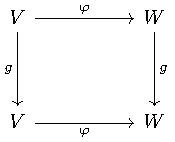
\includegraphics{figures/week-1-diag-1}
\]
commutes for every $g\in G$. (We will call this a \emph{$G$-linear map}
when we want to distinguish it from an arbitrary linear map between the
vector spaces $V$ and $W$). We can then define $\Ker\varphi$,
$\Img\varphi$, and $\Coker\varphi$, which are also $G$-modules.

A \emph{subrepresentation} of a representation $V$ is a vector subspace $W$
of $V$ which is invariant under $G$. A representation $V$ is called
\emph{irreducible} if there is no proper nonzero invariant subspace $W$ of
$V$.

If $V$ and $W$ are representations, so are $V\oplus W$ and $V\otimes W$
with $g(v\otimes w)\coloneqq gv\otimes gw$. Moreover, the $n$th tensor
power $\bigotimes^nV$, the exterior power $\bigwedge^n V$ and symmetric
powers $\Sym^n V$ are subrepresentations of it. The dual $V^*=\Hom(V,\bbC)$
of $V$ is also a representation, though not in the most obvious way: We
want the two representations of $G$ with respect to the natural pairing
between $V$ and $V^*$, so that if $\rho\colon G\to\GL(V)$ is a
representation and $\rho^*\colon G\to\GL(V)$ is its dual, then we have
\begin{equation}
  \label{eq:1:relation-1}
  \langle \rho^*(g)(v^*),\rho(g)(v) \rangle=\langle v^*,v \rangle
\end{equation}
for all $g\in G$, $v\in V$, and $v^*\in V^*$. This in turn forces us to
define the dual representation by
\[
  \rho^*(g)\coloneqq\prescript{\rmt}{}{\rho}(g^{-1})\colon V^*\longrightarrow V^*
\]
for all $g\in G$.

\begin{exercise}
Let us verify that \eqref{eq:1:relation-1} is satisfied by the definition
of $\rho^*$.
\end{exercise}
\begin{proof}
With $\rho^*$ as defined above, choose $g\in G$, $v\in V$ and $v^*\in
V$. Then, we have
\begin{align*}
  \langle \rho^*(g)(v^*),\rho(g)(v) \rangle=\langle v^*,v \rangle
  &=\langle  \rangle\\
  &=
\end{align*}
\end{proof}

Having defined the dual representation of the tensor product of two
representations, it is likewise the case that if $V$ and $W$ are
representations, then $\Hom(V,W)$ is also a representation, via the
identification $\Hom(V,W)=V^*\otimes W$. Unraveling this, if we view an
element of $\Hom(V,W)$ as a linear map $\varphi$ from $V$ to $W$, we have
\[
(g\varphi)(v)=g\varphi(g^{-1}v)
\]
for all $v\in V$. In other words, the definition is such that the diagram
\[
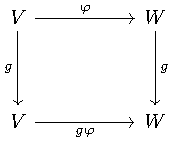
\includegraphics{figures/week-1-diag-2}
\]
commutes. Note that the dual representation is, in turn, a special case of
this: When $W=\bbC$ is the trivial representation, i.e., $gw=w$ for all
$w\in\bbC$, this makes $V^*$ into a $G$-module, with
$g\varphi(v)=\varphi(g^{-1}v)$, i.e.,
$g\varphi=\prescript{\rmt}{}{(g^{-1})}$.

\begin{exercise}
We verify that in general the vector space of $G$-linear maps between two
representations $V$ and $W$ of $G$ is just the subspace $\Hom(V,W)^G$ of
elements of $\Hom(V,G)$ fixed under the action of $G$. We will often denote
this space by $\Hom_G(V,W)$.
\end{exercise}
\begin{proof}
\end{proof}

We have taken the identification $\Hom(V,W)=V^*\otimes W$ as the
definition of the representation $\Hom(V,W)$. More generally, the usual
identities for vector spaces are also true for representations, e.g.,
\begin{align*}
V\otimes(U\oplus W)&=(V\otimes U)\oplus(V\otimes W)\\
\bigwedge^k(V\oplus W)&=\bigoplus_{a+b=k}{\textstyle\bigwedge^a V\otimes\bigwedge^b
  W}\\
{\textstyle\bigwedge^k V^*}&=\left({\textstyle{\bigwedge^kV}}\right)^*
\end{align*}

If $X$ is any finite set and $G$ acts on the left on $X$, i.e.,
$G\to\Aut(X)$ is a homomorphism to the premutation group of $X$, there is
an associated permutation representation: Let $V$ be the vector space with
basis $\{\bfe_x:x\in X\}$, and let $G$ act on $V$ by
\[
  g\cdot\sum a_x\bfe_x\coloneqq\sum a_x\bfe_{gx}.
\]
The regular representation, denoted $R_G$ or simply $R$, corresponds to the
left action of $G$ on itself. Alternatively, $R$ is the space of
complex-valued functions on $G$, where an element $g\in G$ acts on a
function $\alpha$ by $(g\alpha)(h)=\alpha(g^{-1}h)$.

\subsection{Complete Reducibility; Schur's Lemma}
Before we begin classifying the representations of a finite group $G$ we
should try to simplify life by restricting our search
somewhat. Specifically, we have seen that representations of $G$ can be
built up out of other representations by linear algebraic operations, most
simply by taking the direct sum. We should focus, then, on representations
that are ``atomic'' with respect to this operation, i.e., that cannot be
expressed as a direct sum of others; the usual term for such a
representation is \emph{indecomposable}. Happily, this situation is as nice
as it could possibly be: A representation is atomic in this sense if and
only if it is irreducible (i.e., contains no proper subrepresentations);
and every representation is the direct sum of irreducibles, in a suitable
sense uniquely so. The key to all this is
\begin{proposition}
If $W$ is a subrepresentation of a representation $V$ of a finite group
$G$, then there is an elementary invariant subspace $W'$ of $V$, so that
$V=W\oplus W'$.
\end{proposition}
\begin{proof}
  There are two ways of showing this. One can introduce a positive definite
  Hermitian inner product $H$ on $V$ which is preserved by each $g\in G$
  (i.e., such that $H(g\bfv,g\bfw)=H(\bfv,\bfw)$ for all $\bfv,\bfw\in V$,
  $g\in G$). Indeed, if $H_0$ is any Hermitian product on $V$, one gets
  such an $H$ by averaging over $G$:
  \begin{equation}
    \label{eq:1:hermitian-inn-prod}
    H(\bfv,\bfw)\coloneqq\sum_{g\in G}H_0(g\bfv,g\bfw).
  \end{equation}
  Then the perpendicular subspace $W^\perp$ is complementary to $W$ in
  $V$. Alternatively, we can simply choose an arbitrary subspace $U$
  complementary to $W$, let $\pi_0\colon V\to W$ be the projection given by
  the direct sum decomposition $V=W\oplus U$, and average the map $\pi_0$
  over $G$: i.e., take
  \begin{equation}
    \label{eq:1:averaging-map}
    \pi(\bfv)\coloneqq\sum_{g\in G}g(\pi_0(g^{-1}\bfv)).
  \end{equation}
  this will then be a $G$-linear map from $V$ onto $W$, which is
  multiplication by $|G|$ on $W$; its kernel will, therefore, be a subspace
  of $V$ invariant under $G$ and complemnetary to $W$.
\end{proof}

\begin{corollary}
  Any representation is a direct sum of irreducible representations.
\end{corollary}

This property is called complete reducibility, or semisimplicity. We will
see that, for continuous representations, the circle $S^1$, or any compact
group, has this property; integration over the group (with respect to an
invariant measure on the group) plays the role of averaging in the above
proof. The (additive) group $\bbR$ does not have this property: The
representation
\[
  a\longmapsto
  \begin{bmatrix}
    1&a\\0&1
  \end{bmatrix}
\]
leaves the $x$ axis fixed, but there is no complementary subspace. We will
see other Lie groups such as $\SL_n(\bbC)$ that are semisimple in this
sense. Note also that this argument would fail if the vector space $V$ was
over a field of finite characteristic since it might then be the case that
$\pi(\bfv)=\mathbf{0}$ for for $\bfv\in W$. The failure, of complete
reducibility is one  of is one of the things that makes the subject of
modular representations, or representations on vector spaces over finite
fields, so tricky.

The extent to which the decomposition of an arbitrary representation into a
direct sum of irreducible ones is unique is one of the consequences of the
following:

\begin{theorem}[Schur's lemma]
  If $V$ and $W$ are irreducible representations of $G$ and $\varphi\colon
  V\to W$ is a $G$-module homomorphism, the
  \begin{enumerate}[label=\textnormal{(\alph*)},noitemsep]
  \item Either $\varphi$ is an isomorphism, or $\varphi=\mathbf{0}$.
  \item If $V=W$, then $\varphi=\lambda\cdot I$ for some $\lambda\in\bbC$,
    $I$ being the identity.
  \end{enumerate}
\end{theorem}
\begin{proof}
  The first claim follows from the fact that $\Ker\varphi$ and
  $\Img\varphi$ are invariant subspaces. For the second, since $\bbC$ is
  algebraically closed, $\varphi$ must have an eigenvalue $\lambda$, i.e.,
  for some $\lambda\in\bbC$, $\varphi-\lambda I$ has a nonzero kernel. By
  Theorem 1, we must have $\varphi-\lambda I=\mathbf{0}$ so $\varphi=\lambda I$.
\end{proof}

We can summarize what we have shown thus far in
\begin{proposition}
  For any representation $V$ of a finite group $G$, there is a
  decomposition
  \[
    V=V_1^{\oplus a_1}\oplus\dotsb\oplus V_k^{\oplus a_k},
  \]
  where the $V_i$ are distinct irreducible representations. The
  decomposition of $V$ into a direct sum of the $k$ factors is unique, as
  are the $V_i$ that occur and their multiplicities $a_i$.
\end{proposition}
\begin{proof}
It follows from Schur's lemma that if $W$ is another representation of $G$,
with decomposition $W=\bigoplus W_j^{\oplus b_j}$, and $\varphi\colon V\to
W$ is a map of representations, then $\varphi$ must map the factor
$V_i^{\oplus a_i}$ into that factor $W_j^{\oplus b_j}$ for which $W_j\simeq
V_i$; when applied to the identity map of $V$ to $V$, the stated uniqueness
follows.
\end{proof}

%%% Local Variables:
%%% mode: latex
%%% TeX-master: "../MA598-Lie-Groups"
%%% End:
